\documentclass[../main]{subfiles}
\graphicspath{{\subfix{../Images/}}}

\begin{document}

\section*{Załącznik nr 1: System wbudowany}\addcontentsline{toc}{section}{Załącznik nr 1: System wbudowany}\label{sec:zalacznik-1}

Skoro nie ma jednoznacznej definicji pojęcia "system wbudowany" - należy określić definicję, która jest
wykorzystywana w tej pracę.

System wbudowany jest systemem, to znaczy ma cechy systemu: jest złożony z więcej niż jednego elementu,
jest funkcjonalnie niezależny od środowiska i posiada możliwość reagowania (tzn. odbierania,
przetwarzania i odpowiedzi) na bodźce zewnętrzne. "wbudowany" oznacza, że system jest częścią innego
systemu fizycznie i/lub
funkcjonalnie.

Natomiast przełożyć tą definicję na dziedzinę elektroniki i informatyki można w następujący sposób:
system wbudowany — jest to system komputerowy składający się z jednostki obliczeniowej i modułów
wejścia/wyjścia (tzn. może reagować na bodźce zewnętrzne), mający wszystkie narzędzia (w tym
oprogramowanie) dla spełnienia pewnej, zdefiniowanej funkcji (więc może być wyodrębniony) i będący
częścią większego systemu.
% TODO: Nie cytuję tu rzadnej książki ani normy, bazuję sie na swojej wiedzę, ale agólnie ta definicja jest podobna od książki do książki.

\section*{Załącznik nr 2: ARM TrustZone}\addcontentsline{toc}{section}{Załącznik nr 2: ARM TrustZone}\label{sec:zalacznik-2}
\begin{figure}
    \centering
    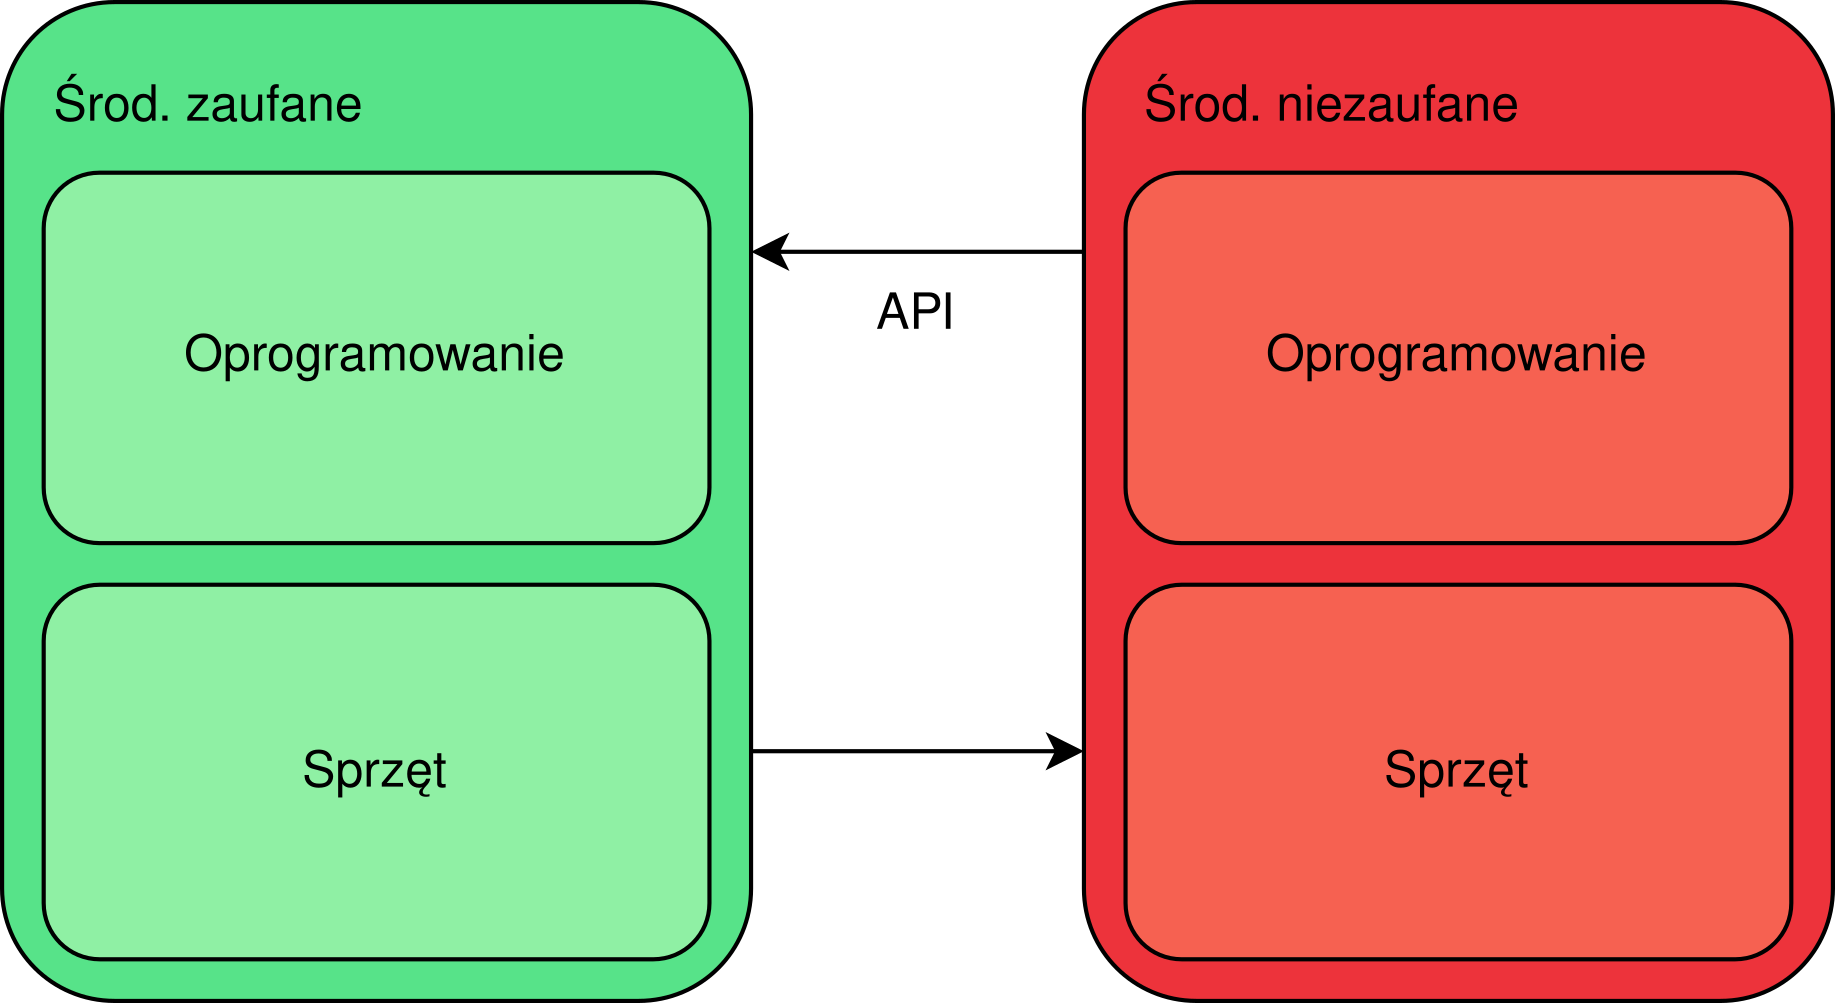
\includegraphics[width=0.75\textwidth]{Images/trustzone-m.png}
    \caption{TrustZone dla architektury \acrshort{arm} v8-M. Kolorami są dodatkowo odznaczone środowiska: zielony — środowisko zaufane, czerwony — środowisko niezaufane}
    \label{fig:trustzone-m}
\end{figure}
\begin{figure}
    \centering
    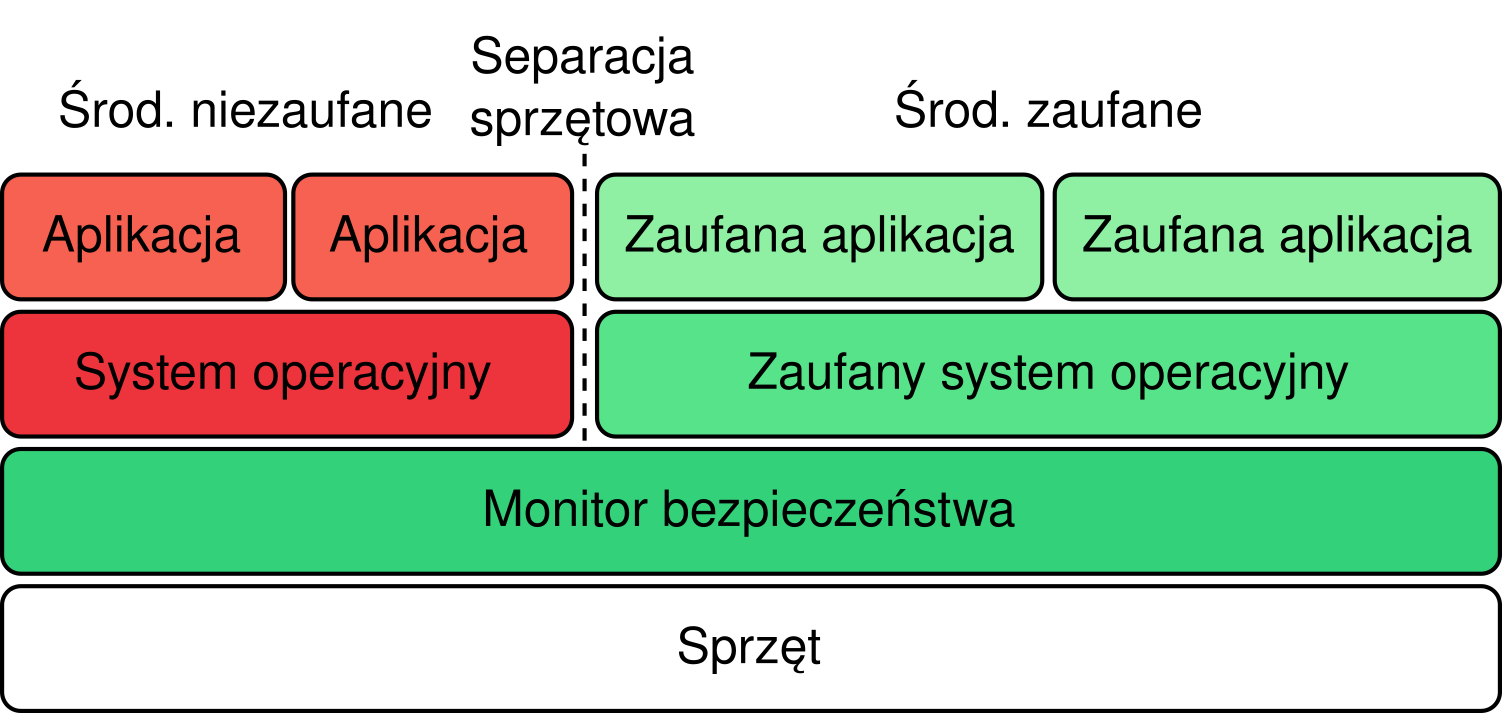
\includegraphics[width=0.75\textwidth]{Images/trustzone-a.png}
    \caption{TrustZone dla architektury \acrshort{arm} v8-A. Kolorami są dodatkowo odznaczone środowiska: zielony — środowisko zaufane, czerwony — środowisko niezaufane}
    \label{fig:trustzone-a}
\end{figure}

Koncept technologi TrustZone bazuję się na podziale sprzętowym środowiska (pamięci i innych zasobów) na
środowisko zaufane i niezaufane (\cref{fig:trustzone-m} i
\cref{fig:trustzone-a}), co jest robione za pomocą rozszerzeń do architektur ARMv8-A i
ARMv8-M dotyczących \acrshort{bsa} i \acrshort{isa}.

Dla architektury ARMv8-A został dodany \acrshort{el}3, w którym jest zamieszczony monitor bezpieczeństwa
(\cref{fig:trustzone-a}), realizowany przez oprogramowanie \acrshort{arm}'owe Trusted
Firmware A (referencyjna implementacja monitoru bezpieczeństwa). Faktycznie ten monitor bezpieczeństwa
jest pewnym mostem przekazującym polecenia ze środowiska niezaufanego do środowiska zaufanego oraz
przełączający procesor w bezpieczny tryb za pomocą \acrshort{smccc}.
\cite{smccc}\cite{trustzoneaarch64} % TODO: automatic images indexing

Dla architektury ARMv8-M zostały dodane rozszerzenia pozwalające na separację środowiska zaufanego od
niezaufanego (\cref{fig:trustzone-m}) za pomocą modułów \acrshort{sau} i \acrshort{idau},
oraz instrukcji dla komunikacji pomiędzy środowiskami: \acrshort{isa} SG, BXNS i BLXNS.
\cite{trustzonearmv8m}

\section*{Załącznik nr 3: Wirtualizacja}\addcontentsline{toc}{section}{Załącznik nr 3: Wirtualzacja}\label{sec:zalacznik-3}

Wirtualizacja jest technologią wprowadzającą separację środowisk z oprogramowaniem poprzez tworzenie
tzw. \acrshort{vm} zarządzanych przez \acrshort{vmm} (\cref{fig:virt}). Typy separacji używane w
wirtualizacji: separacja pamięciowa (poprzez translację pamięci), separacja sygnałowa (przekierowywanie
przerwań) i separacja stanów (przełączanie kontekstu).

Celą separacji pamięciowej jest przypisanie do każdej \acrshort{vm} przedziału adresu pamięci (kodu
programu i urządzeń peryferyjnych, ponieważ rejestry tych urządzeń są zmapowane do pamięci; ang. memory
mapped peripherals) i wychwytywanie wszystkich prób manipulacji pamięcią nieprzypisaną do tej
\acrshort{vm}. W architekturach \acrshort{arm} tym się zajmuje \acrshort{mmu}, który, zaczynając od
\acrshort{arm}v8, posiada dwa poziomy translacji: z poziomu aplikacji (\acrshort{va}), do poziomu
systemu operacyjnego (\acrshort{ipa}) i do poziomu hiperwizora (\acrshort{pa})
\cite{armv8amemtranslation}.

Celą separacji sygnałowej jest podział i przekierowywanie przerwań sprzętowych pomiędzy \acrshort{vm}.
Każda \acrshort{vm} ma przepisany podzbiór urządzeń peryferyjnych za pomocą separacji pamięci, te
urządzenia mogą generować przerwania, za przekierowywanie których jest odpowiedzialny hiperwizor i
kontroler przerwań (w przypadku \acrshort{arm}'u to jest \acrshort{gic}).

Celą separacji stanów jest sprzętowy podział wykonywanych programów i przypisanie do nich pewnych
poziomów uprawnień. Dokładniej to jest opisane w \hyperref[sec:zalacznik-4]{załączniku nr 4}.

Przy czym, typowo hiperwizor jest zaprojektowany w taki sposób, że przy użyciu wszystkich tych rodzai separacji, aplikacja (lub system operacyjny), uruchomiana na tym hiperwizorze, wcale nie musi wiedzieć że jest uruchomiana nie wprost na rzeczywistym sprzęcie. Taki rodzaj wirtualizacji jest nazywany wirtualizacja natywną (ang. native virtualization, także ang. full virtualization, lub ang. hardware-accelerated virtualization).

W przypadku, kiedy sprzęt nie posiada dedykowanych narzędzi do zapewnienia jakiegoś z rodzajów separacji, można skorzystać z tzw. parawirtualizacji (ang. paravirtualization). W takim przypadku aplikacja, która jest uruchamiana na hiperwizorze jest modyfikowana w sposób taki, aby ona wiedziała, że jest uruchomiona nie na realnym sprzęcie a na wirtualnym i wiedziała o obecności hiperwizora. Przykładem może być separacja pamięciowa. Typowo próba otrzymania dostępu do zabronionej sekcji pamięci RAM jest wykrywana przez \acrshort{mmu}, w przypadku nieobecności tego modułu, uruchamiana aplikacja jest modyfikowana i wszystkie instrukcje odczytujące coś z pamięci są podmieniane na zestaw instrukcji, który powoduje komunikat do hiperwizora ze sprawdzeniem dostępów.

\section*{Załącznik nr 4: Przełączanie stanu i kontekstu, definicja procesu}\addcontentsline{toc}{section}{Załącznik nr 4: Przęłączanie stanu i kontekstu, definicja procesu}\label{sec:zalacznik-4}

\begin{figure}
    \centering
    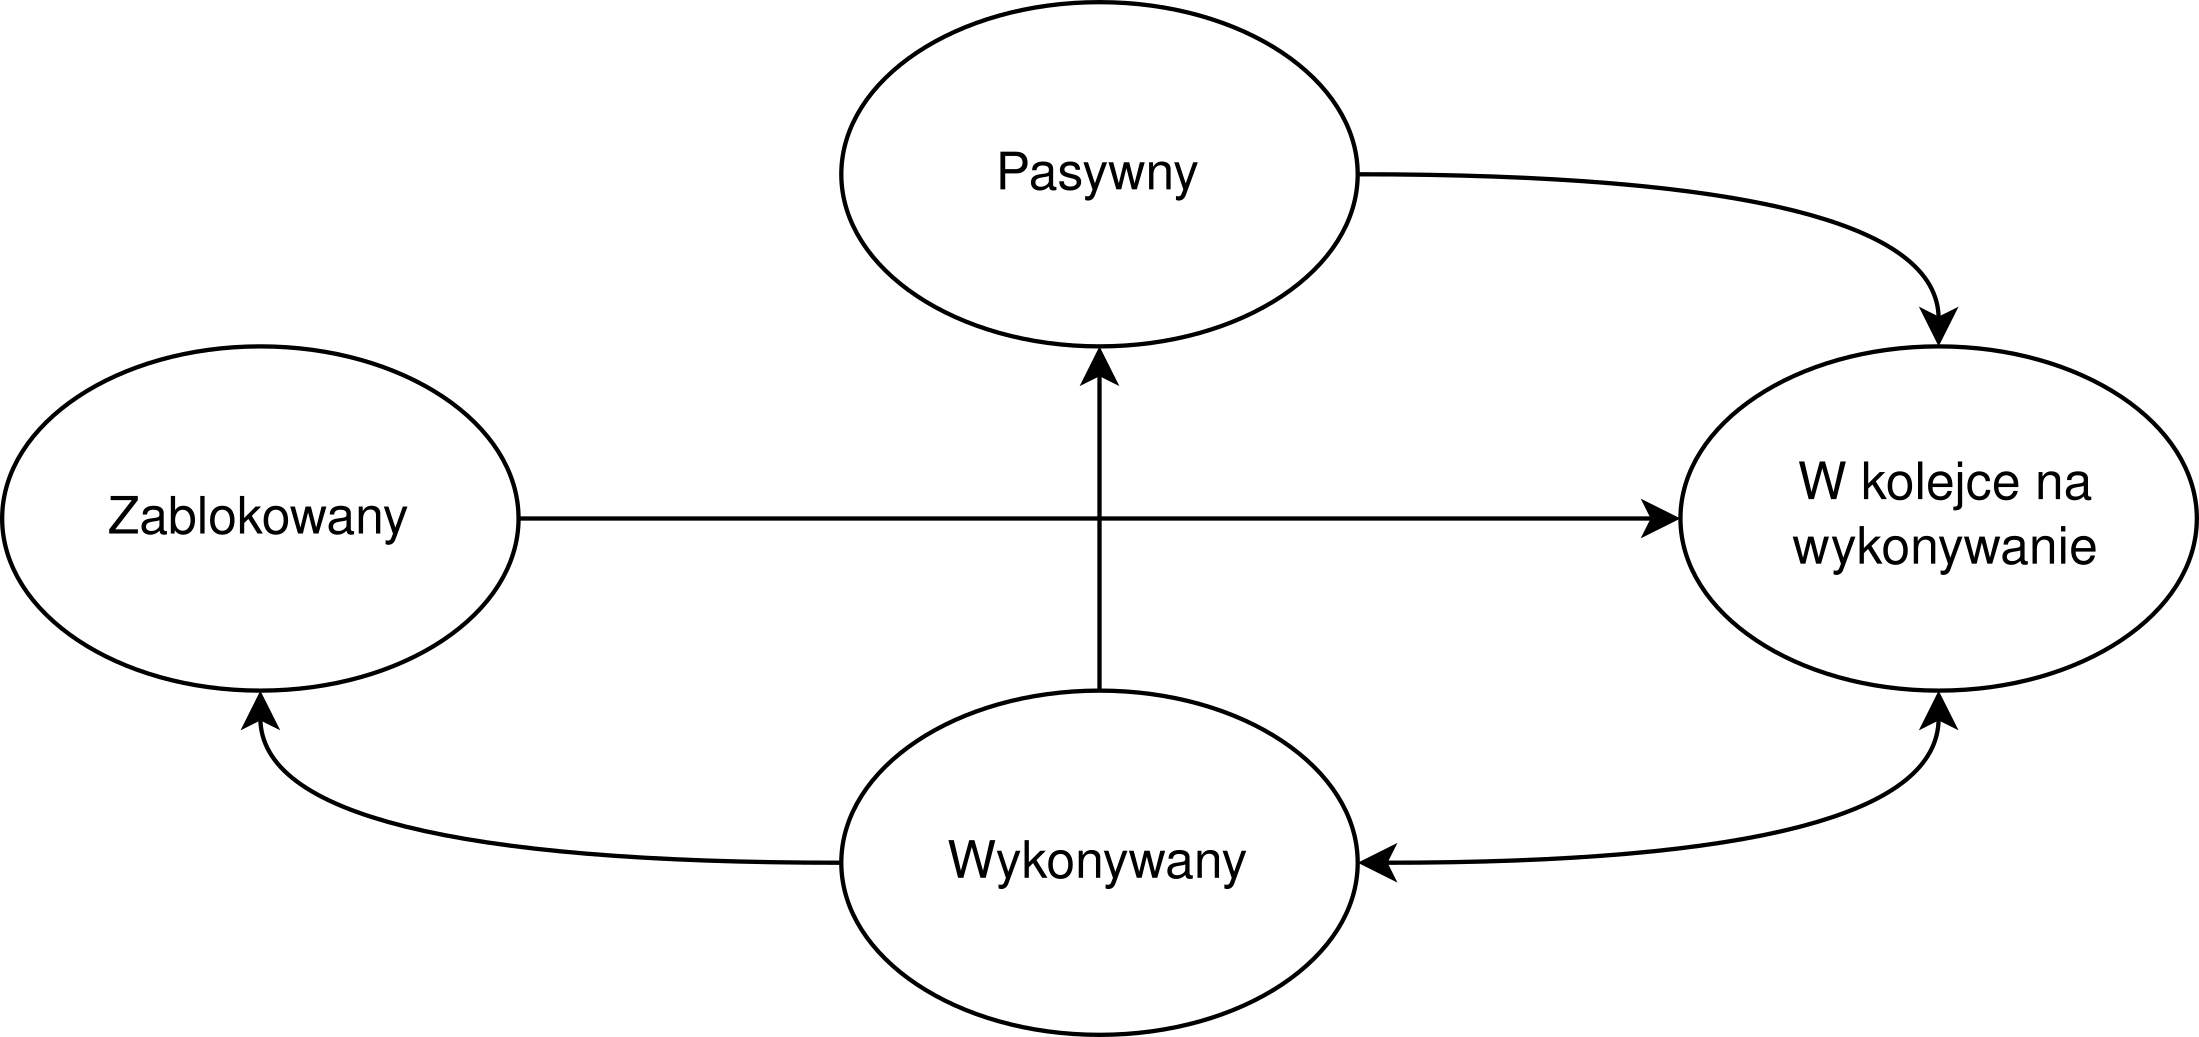
\includegraphics[width=0.85\textwidth]{Images/process-states.png}
    \caption{Ogólny graf stanów procesu}
    \label{fig:process-states}
\end{figure}

Na początku należy oddzielić pojęcie programu od pojęcia procesu. Programem, w przypadku oprogramowania, jest lista instrukcji do wykonania przechowywana w jakimkolwiek miejscu. Program nie posiada, żadnego stanu, on po prostu istnieje. Natomiast procesem jest program z przydzielonym stanem. Każdy stan procesu może zawierać dodatkowe dane, np. priorytet, zasoby, połączenia z innymi procesami i tak dalej. Na \cref{fig:process-states} jest pokazany najbardziej popularne stany procesu i przejścia pomiędzy nimi.

Stan wykonywanego oprogramowania jest określany poprzez następujące elementy:

\begin{itemize}
    \item Zawartości rejestrów ogólnego przeznaczenia: zawierają wyniki wykonywania ostatnich
    instrukcji;
    \item Rejestry wskazujące na adres następnej komendy (PC w architekturach \acrshort{arm}'owych),
    adres powrotu (LR w architekturach \acrshort{arm}'owych) i adres aktualnie używanego stosu (MSP
    lub PSP w architekturach \acrshort{arm}): określają "kierunek" (tzn. co będzie wykonane następne,
    gdzie wrócić po wykonaniu i tak dalej) wykonywanych instrukcji oprogramowania;
    \item Zawartość aktualnie używanego stosu: tak samo jak i poprzedni punkt, określa "kierunek"
    wykonywania instrukcji oprogramowania, przechowuje historie wykonywanych instrukcji oprogramowania
    (np. przy przerwaniu, do niego są zapisywane pewne rejestry, które po zakończeniu przerwania są
    odczytywane z powrotem, pozwalając na wznowienie wykonywanego programu);
    \item Rejestry systemowe (np. PSR i rejestry masek przerwań w architekturach \acrshort{arm}'owych):
    określają między innymi tryb jednostki obliczeniowej, w którym program jest wykonywany, co z kolei
    określa poziom dostępu do zasobów sprzętowych.
\end{itemize}

Z powyższego wynika, że stan wykonywanego oprogramowania — to jest zbiór pewnych wartości
przechowywanych w rejestrach jednostki obliczeniowej, co oznacza, że przełączenie stanów jest robione
sprzętowo, przez jednostkę obliczeniową (ponieważ oprogramowanie nie ma dostępu zapisu lub odczytu do
wszystkich rejestrów jednostki obliczeniowej).

Z kolei przełączenie stanów — to jest proces, kiedy stan aktualnie wykonywanego oprogramowania jest
zapisywany (w stos przynależącego do tego oprogramowania) i podmieniany na stan przynależący do innego
oprogramowania (który jest odczytywany ze stosu uruchamianego oprogramowania). Występuje to podczas
zmiany trybu jednostki obliczeniowej, ponieważ każdy tryb jednostki obliczeniowej ma własny stos.

\begin{figure}[h]
    \centering
    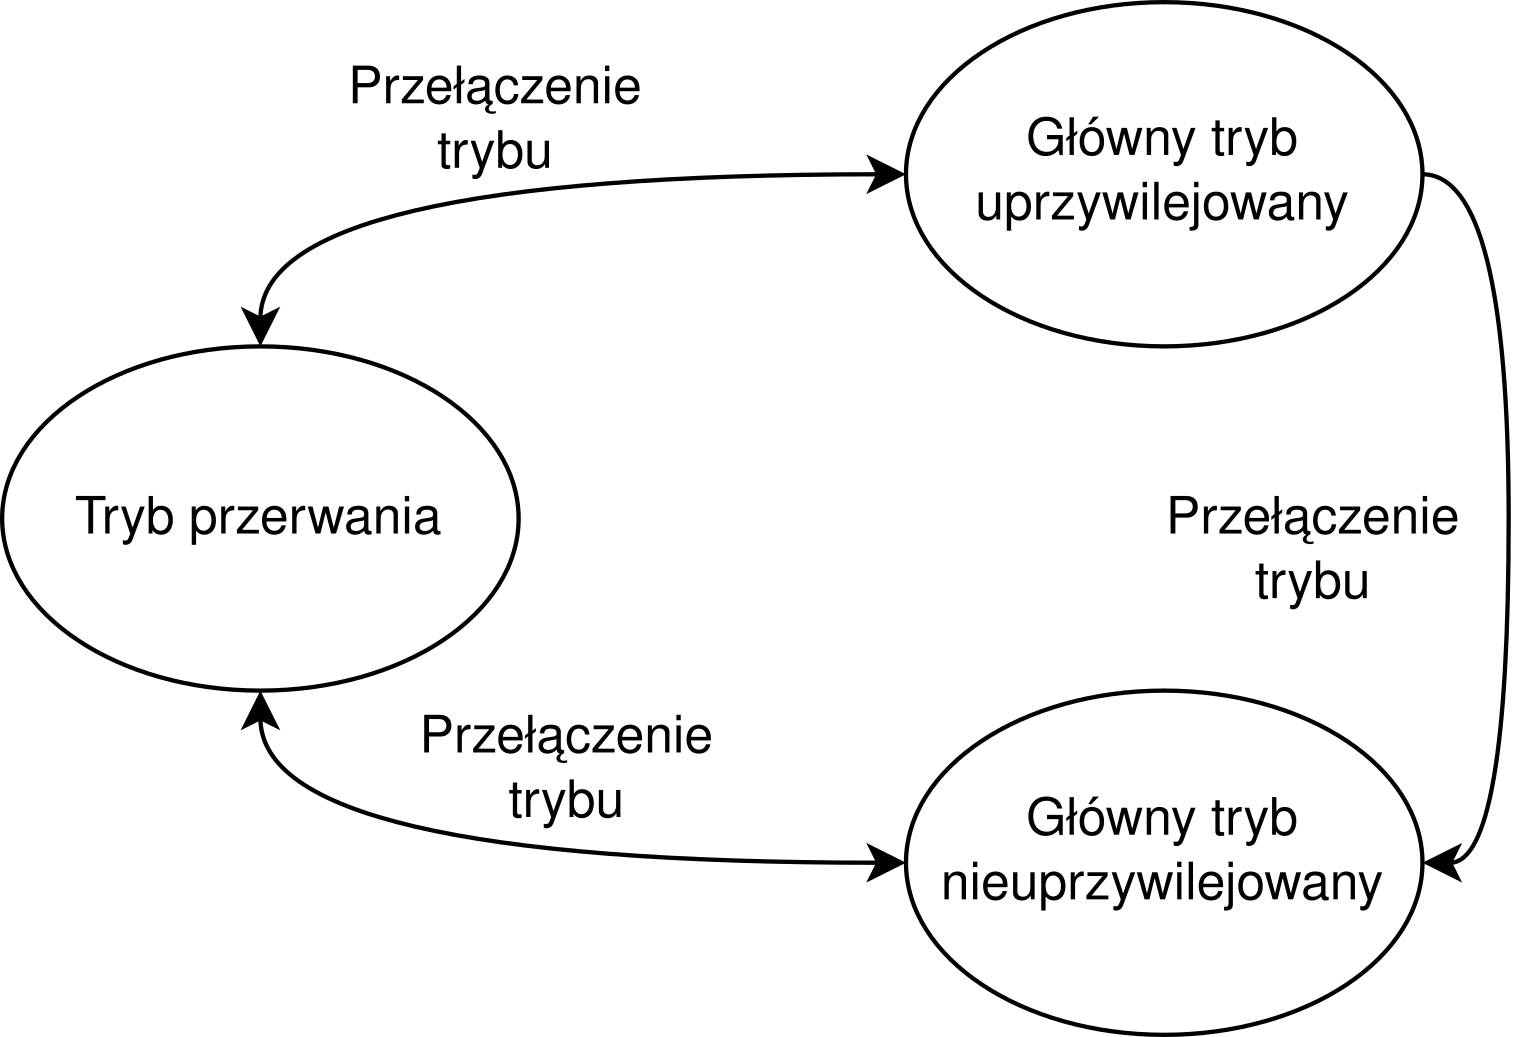
\includegraphics[width=0.7\textwidth]{Images/armv8m-modes.png}
    \caption{Tryby procesora zbudowanego na podstawie architektury \acrshort{arm}v8-\acrshort{m}
    \cite{armv8mintro}}
    \label{fig:armv8-m-modes}
\end{figure}

Na \cref{fig:armv8-m-modes} są pokazane tryby jednostki obliczeniowej zbudowanej na podstawie
architektury \acrshort{arm}v8-\acrshort{m}. Taka jednostka posiada trzy tryby z dwoma poziomami
dostępu: tryb główny (główny uprzywilejowany i główny nieuprzywilejowany) i tryb przerwania. Każdy z
tych trybów ma swój stos, w którym jest przechowywany stan aktualnie wykonywanego oprogramowania.
Adres na każdy ze stosów jest przechowywany w rejestrach MSP i PSP \cite{armv8mintro}.

Natomiast kontekst programu jest pojęciem definiowanym przez poszczególną implementację oprogramowania
systemowego (system operacyjny bądź hiperwizor) i zawiera w sobie opisany wyżej stan programu oraz
dodatkowe dane, interpretowane przez oprogramowanie systemowe (np. czas jednostki obliczeniowej, który
był użyty przez ten program, lub priorytet).

Stąd przełączenie kontekstu oznacza, że nie jednostka obliczeniowa jest odpowiedzialna za wybór i
uruchomienie pewnego programu, tylko oprogramowanie systemowe.

Na \cref{fig:armv8-m-context-switch} jest pokazany przykładowy przebieg takiego przełączenia dla
architektury \acrshort{arm}v8-\acrshort{m}. Przełączenie kontekstu następuje podczas wykonywania kodu
systemu operacyjnego, tzn. kiedy jednostka obliczeniowa znajduje się w trybie głównym uprzywilejowanym
(\cref{fig:armv8-m-modes}), co oznacza, że przed przełączeniem kontekstu następuje przełączenie
stanów, podczas którego jednostka obliczeniowa przełącza się z wykonywania kodu aktualnego programu na
wykonywanie kodu systemu operacyjnego (tzn. przechodzi z trybu głównego nieuprzywilejowanego do trybu
głównego uprzywilejowanego, \cref{fig:armv8-m-modes}). Natomiast po przełączeniu kontekstu następuje
przełączenie stanów, podczas którego jednostka obliczeniowa przełącza się z wykonywania kodu systemu
operacyjnego na wykonywanie kodu programu zaproponowanego przez system operacyjny podczas przełączenia
kontekstu programu (tzn. przechodzi z trybu głównego uprzywilejowanego do trybu głównego
nieuprzywilejowanego).

\section*{Załącznik nr 5: Zasób jednostki obliczeniowej}\addcontentsline{toc}{section}{Załącznik nr 5: Zasób jednostki obliczeniowej}\label{sec:zalacznik-5}

\begin{figure}[h]
    \centering
    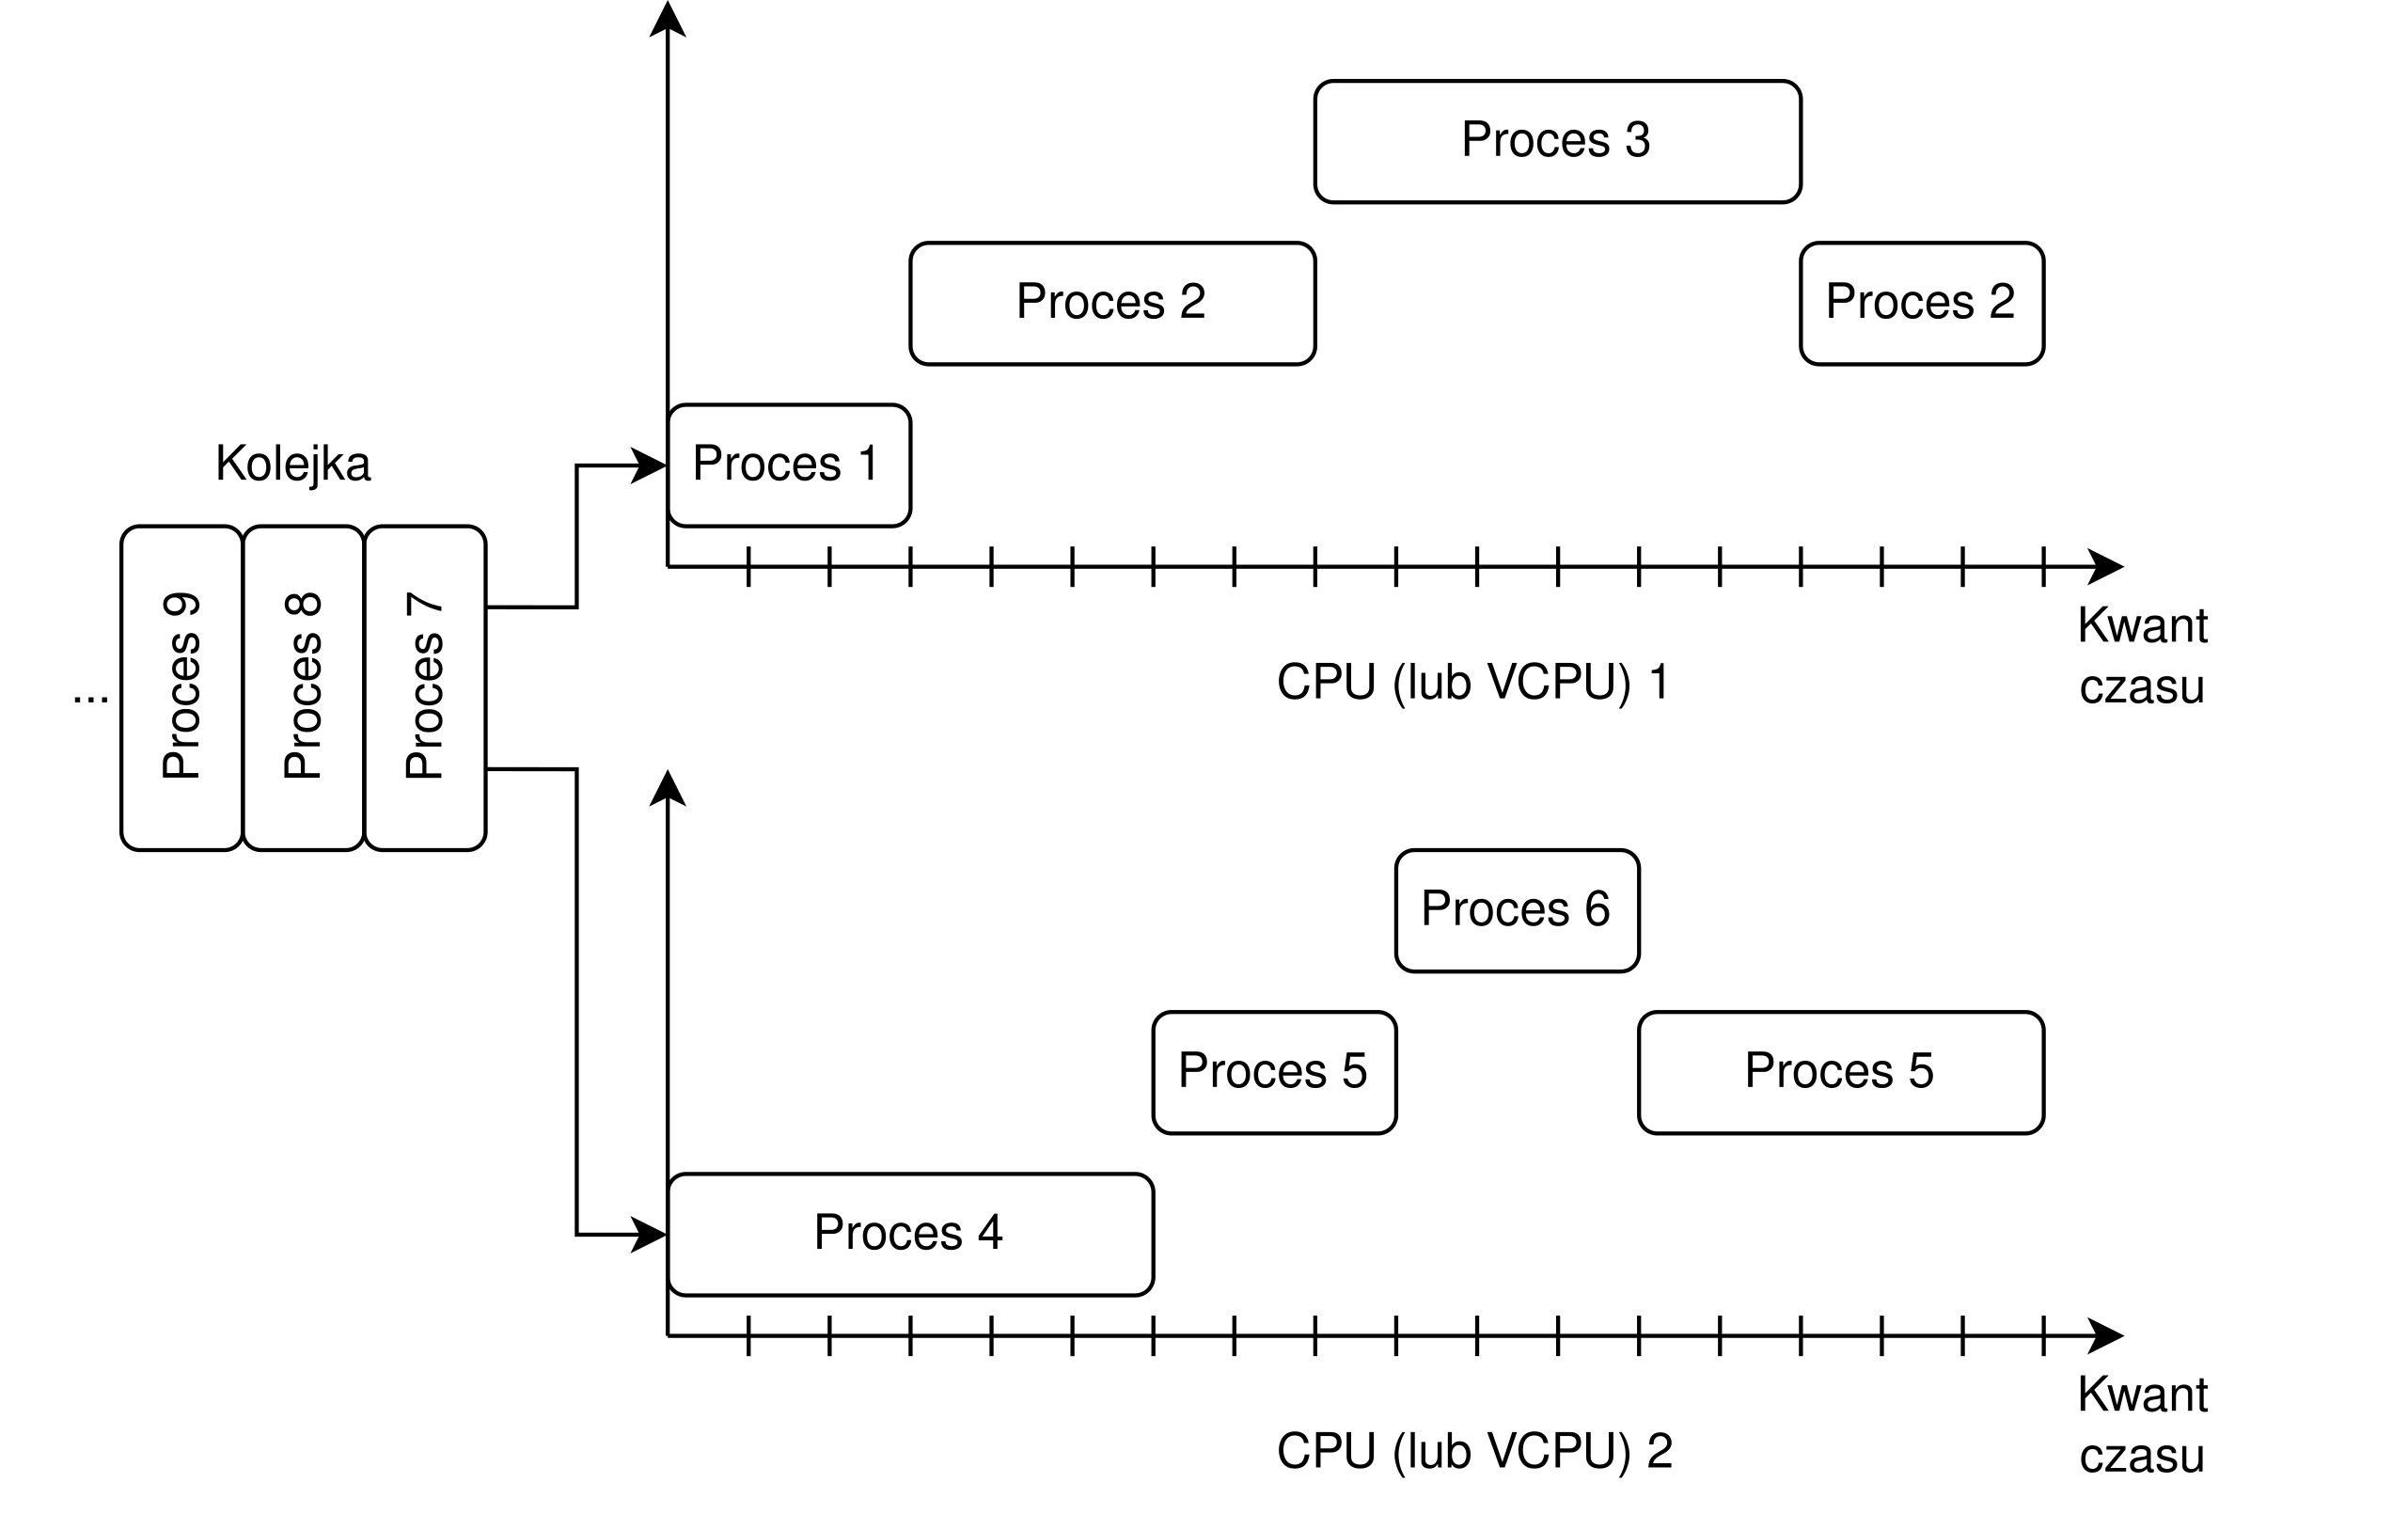
\includegraphics[width=0.95\textwidth]{Images/time-sharing.png}
    \caption{Współdielenie zasobów jednostek obliczeniowych przez wiele procesów w technologii \acrshort{amp}}
    \label{fig:time-sharing}
\end{figure}

Jednostka obliczeniowa jest pewnym systemem przyjmującym instrukcje, wykonującym je i podającym wynik. Więc podstawową wielkością będzie czas wykonania jednej instrukcji (w przypadku architektury \acrshort{risc} większość instrukcji są wykonywane w przedziale jednego okresu zegara zasilającego jednostkę obliczeniową).

Każdy program wykonywany przez jednostkę obliczeniową jest listą instrukcji, i każdemu programu zależy, aby ta list instrukcji była wykonana jak najszybciej, czyli idealnie jakby jedna jednostka obliczeniowa wykonywała tylko jeden program. Z tego wynika, że programy walczą o czas, na który im pozwolono używać jednostki obliczeniową do wykonania swoich instrukcji. Finalnie mamy — zasobem jednostki obliczeniowej jest czas.

Czas ten można podzielić pomiędzy programami w różny sposób, za to akurat odpowiada nadzorca w oprogramowaniu systemowym.

W przypadku kiedy mamy kilka jednostek obliczeniowych dostępnych dla wszystkich programów, zorganizować zarządzaniem ich zasobów można na dwa sposoby: przydzielać każdemu programu czas oddzielnej jednostki obliczeniowej (techniki \acrshort{amp}) lub połączyć zasoby wszystkich jednostek obliczeniowych i przydzielać jednemu programu pewną część (techniki \acrshort{smp}).

W przypadku wirtualizacji programom są udostępniane \acrshort{vcpu}. Są to w pewny sposób przerobione przez hiperwizor zasoby realnej jednostki obliczeniowej.

Na \cref{fig:time-sharing} jest pokazany przykład współdzielenia zasobów jednostek obliczeniowych przez wiele procesów technologii \acrshort{amp}. Każdemu procesowi jest przypisana pewna część zasobów obliczeniowych reprozentowana przez ilość kwantów czasu (ang. time slice; najmniejsza możliwa ilość czasu jednostki obliczeniowej, którą można przypisać procesu w niektórych realizacja oprogramowania systemowego).

Stąd można zrobić trzy wnioski:

\begin{enumerate}
    \item Zasobem jednostki obliczeniowej jest jej czas;
    \item Czas może być przypisywany bezpośrednio, lub on może być podzielony przez oprogramowanie systemowe na pewne minimalne odcinki: kwanty czasu;
    \item W przypadku obecności wielu jednostek obliczeniowych, zarządzanie ich zasobami odbywa się zgodnie z technikami \acrshort{amp} lub \acrshort{smp}.
\end{enumerate}

\end{document}
